\chapter{Appendix}\label{ch:appendix_c}

\section{Additional data}
Additional data, including the raw data and the code used to generate the figures in this thesis, can be obtained on request from
Synaptica B.V. See copyright statement for contact details.

\section{Additional figures}
Additional figures for the results of the noise and recurrent connection variants are shown in the following pages.
Representative figures are shown in the results section.
\pagebreak
\subsection{External Noise variants: DPB percentage matrices}\label{subsec:DPB_percentage_matrices}
% Page 1
\begin{figure}[!ht]
    \centering
    % Row 1
    \begin{subfigure}{0.48\textwidth}
        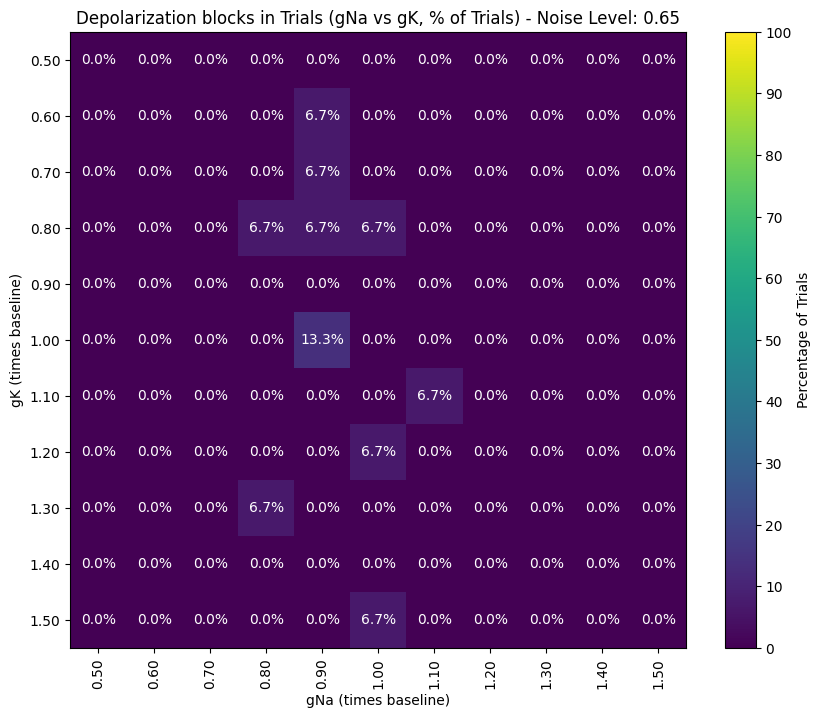
\includegraphics[width=\linewidth]{DPB_percentage_matrices/DPB_percentage_noise_0.65.png}
        \caption{} % Optional caption
    \end{subfigure}\hfill
    \begin{subfigure}{0.48\textwidth}
        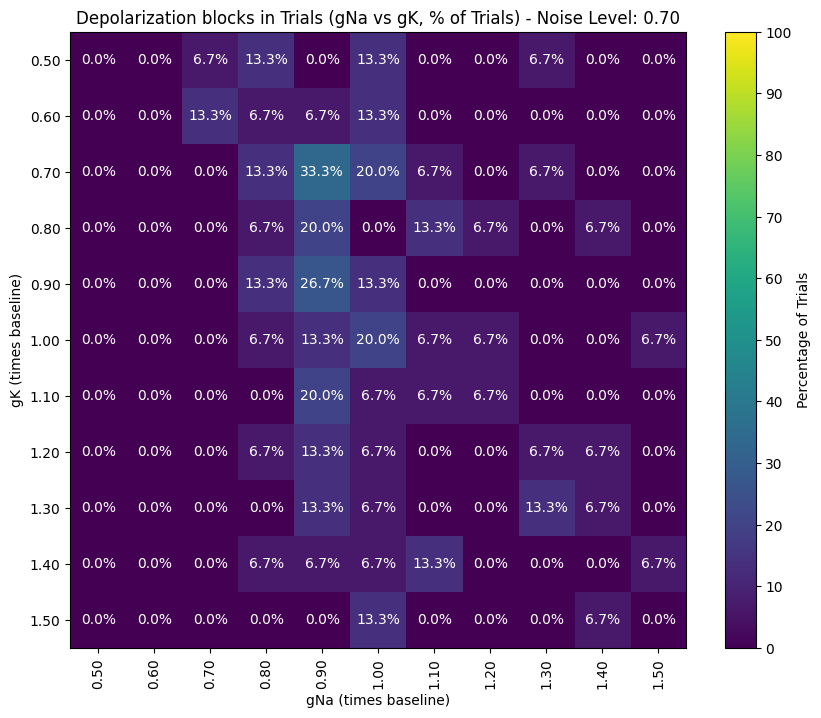
\includegraphics[width=\linewidth]{DPB_percentage_matrices/DPB_percentage_noise_0.70.png}
        \caption{} % Optional caption
    \end{subfigure}

    \bigskip % Adds vertical space between the rows

    % Row 2
    \begin{subfigure}{0.48\textwidth}
        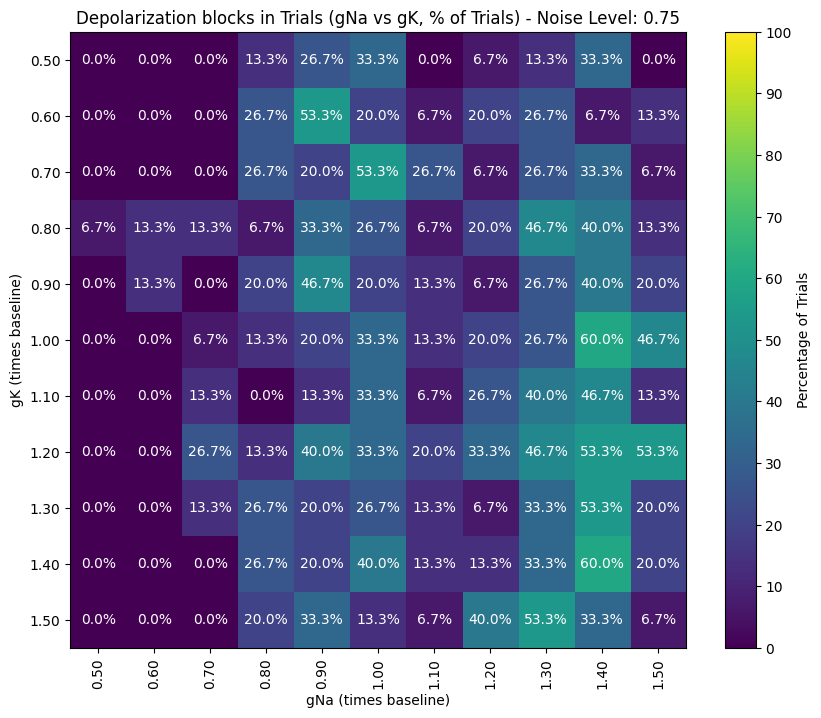
\includegraphics[width=\linewidth]{DPB_percentage_matrices/DPB_percentage_noise_0.75.png}
        \caption{} % Optional caption
    \end{subfigure}\hfill
    \begin{subfigure}{0.48\textwidth}
        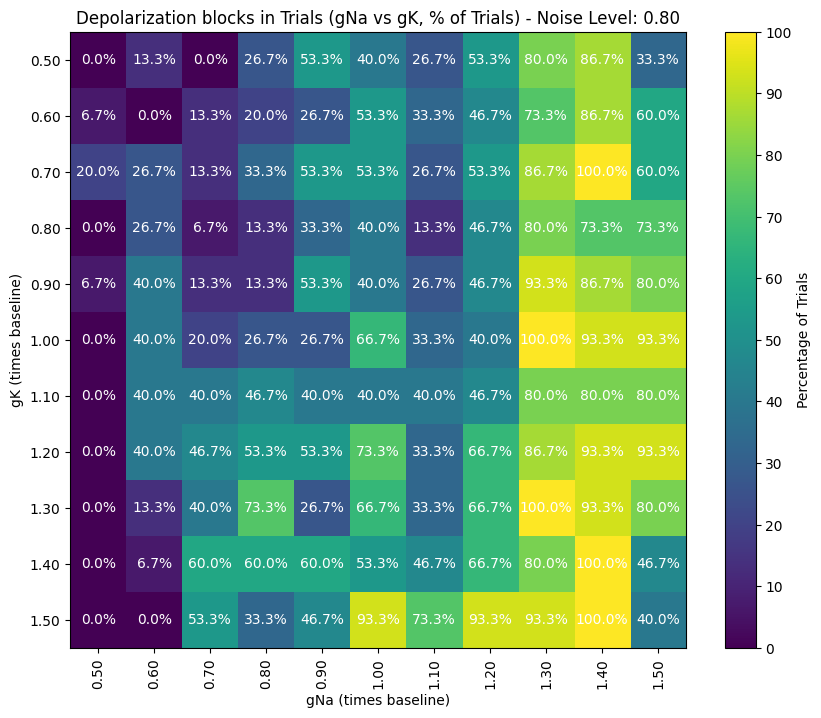
\includegraphics[width=\linewidth]{DPB_percentage_matrices/DPB_percentage_noise_0.80.png}
        \caption{} % Optional caption
    \end{subfigure}

    \caption[DPB percentage matrices (all)]{Percentage of trials where depolarization block events occurred for all tested noise conditions.
        The x-axis shows all the sodium conductance changes in pyramidal cells, whereas the y-axis shows the potassium conductance changes in pyramidal cells.
        Modifications to pyramidal cells were applied to all compartments.
        The color intensity scales from 0 to 100 \%, where high-intensity yellow equals a higher amount of DPB events in a condition.
        The images are labeled from low noise to higher noise (a through k), respectively.}\label{fig:dpb_percentage_matrices_all}
\end{figure}

% Page 2
\begin{figure}[H] \ContinuedFloat% continue the figure from the previous page
    \centering
    % Row 3
    \begin{subfigure}{0.48\textwidth}
        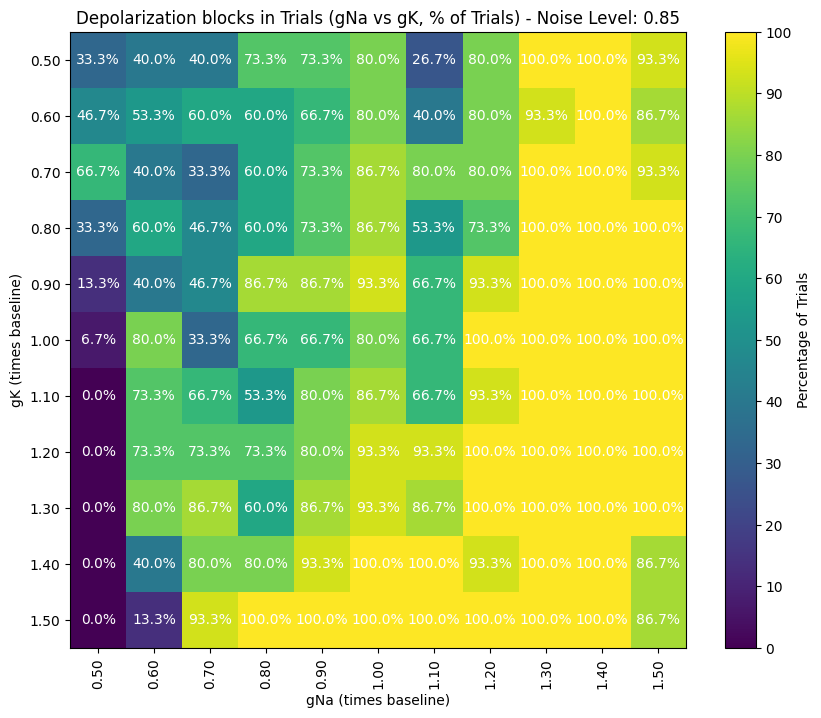
\includegraphics[width=\linewidth]{DPB_percentage_matrices/DPB_percentage_noise_0.85.png}
        \caption{} % Optional caption
    \end{subfigure}\hfill
    \begin{subfigure}{0.48\textwidth}
        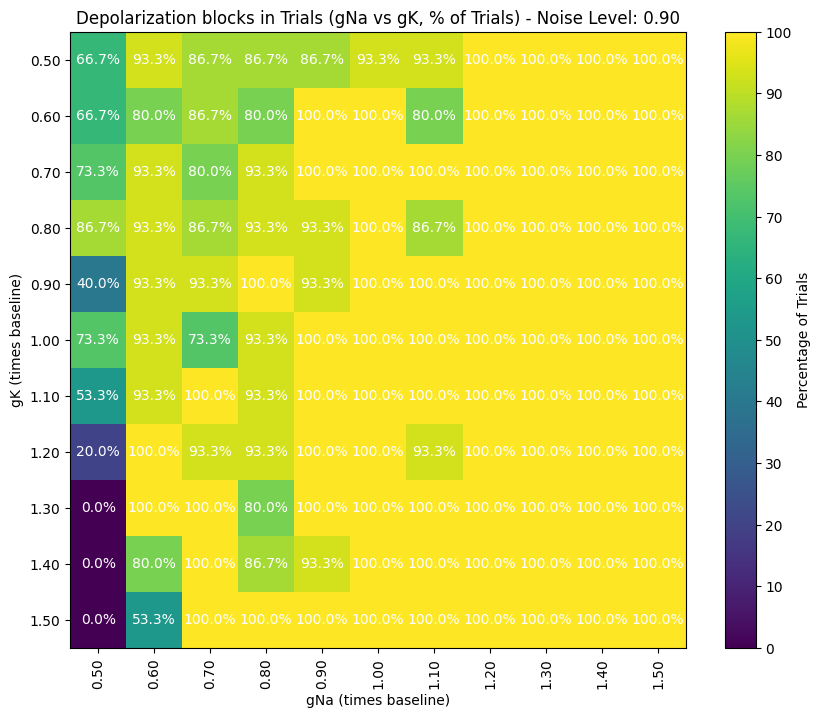
\includegraphics[width=\linewidth]{DPB_percentage_matrices/DPB_percentage_noise_0.90.png}
        \caption{} % Optional caption
    \end{subfigure}

    \bigskip % Adds vertical space between the rows

    % Row 4
    \begin{subfigure}{0.48\textwidth}
        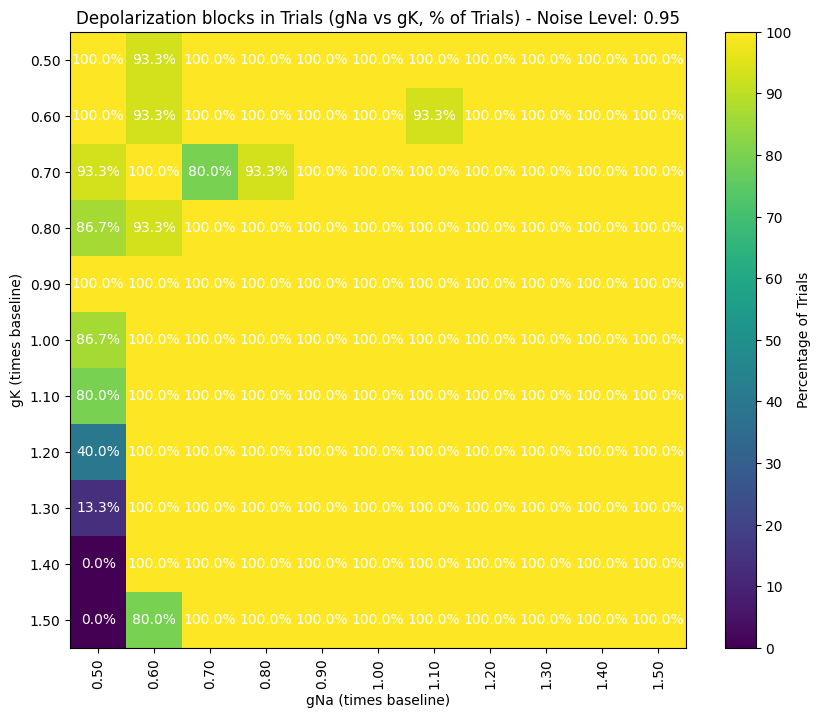
\includegraphics[width=\linewidth]{DPB_percentage_matrices/DPB_percentage_noise_0.95.png}
        \caption{} % Optional caption
    \end{subfigure}\hfill
    \begin{subfigure}{0.48\textwidth}
        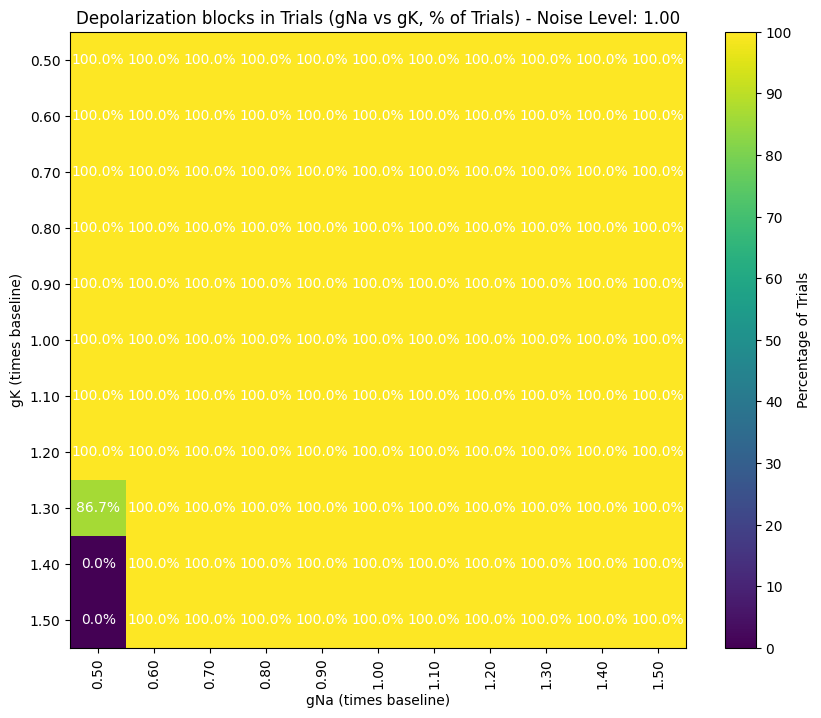
\includegraphics[width=\linewidth]{DPB_percentage_matrices/DPB_percentage_noise_1.00.png}
        \caption{} % Optional caption
    \end{subfigure}
\end{figure}

% Page 3
\begin{figure}[H] \ContinuedFloat% continue the figure from the previous page
    \centering
    % Row 5
    \begin{subfigure}{0.48\textwidth}
        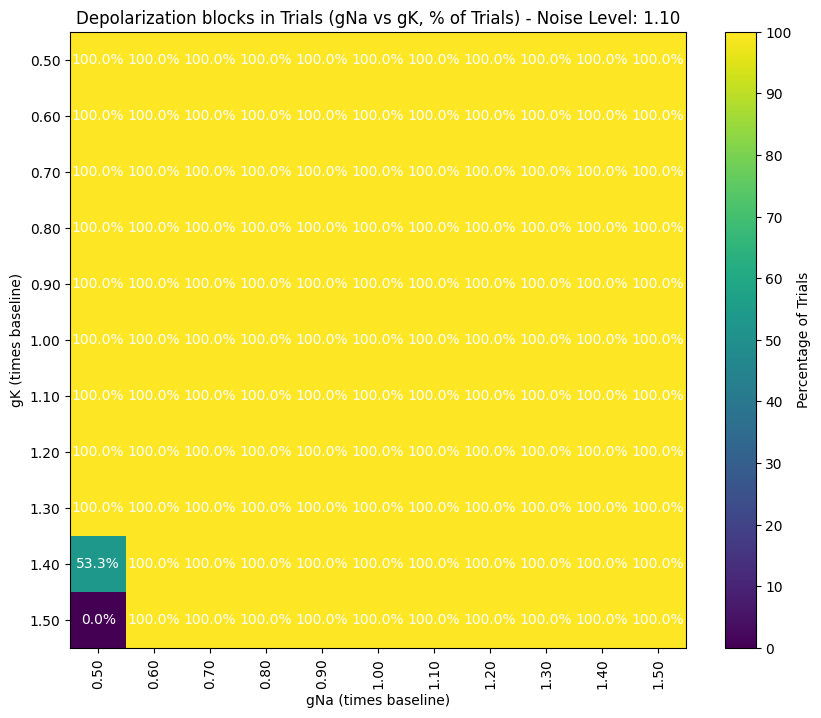
\includegraphics[width=\linewidth]{DPB_percentage_matrices/DPB_percentage_noise_1.10.png}
        \caption{} % Optional caption
    \end{subfigure}\hfill
    \begin{subfigure}{0.48\textwidth}
        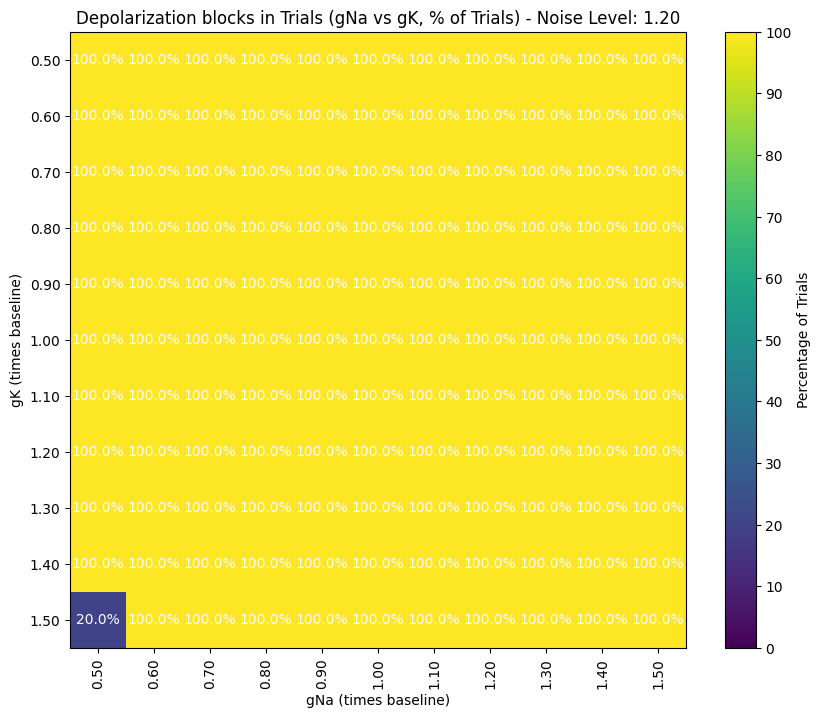
\includegraphics[width=\linewidth]{DPB_percentage_matrices/DPB_percentage_noise_1.20.png}
        \caption{} % Optional caption
    \end{subfigure}

    \bigskip % Adds vertical space between the rows

    % Row 6
    \begin{subfigure}{0.48\textwidth}
        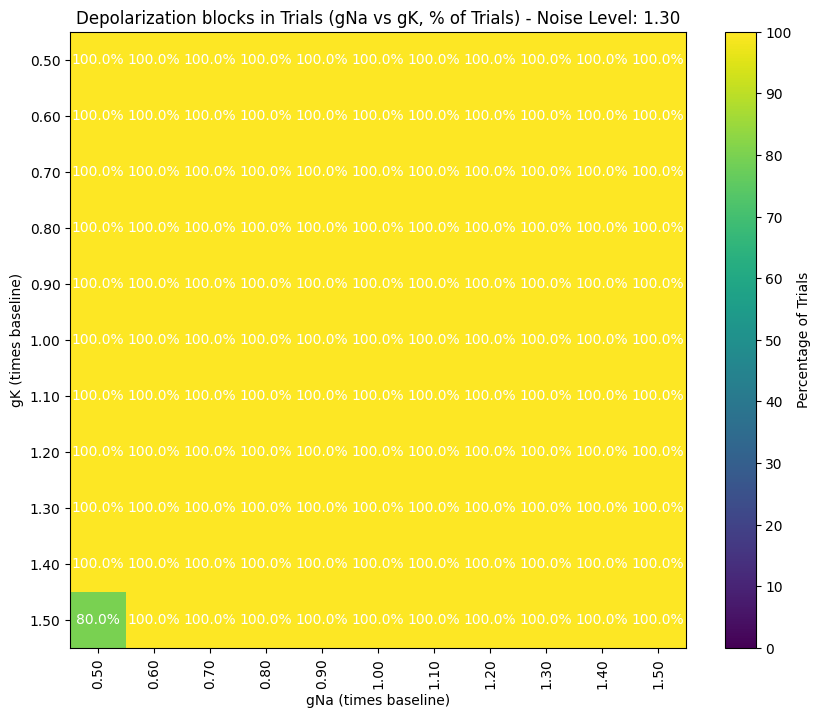
\includegraphics[width=\linewidth]{DPB_percentage_matrices/DPB_percentage_noise_1.30.png}
        \caption{} % Optional caption
    \end{subfigure}
    % Since the last row has only one image, you might adjust its position or add another sub-figure if needed.
\end{figure}
\pagebreak

\subsection{External Noise variants: DPB delay matrices}\label{subsec:DPB_delay_matrices}
% Page 1
\begin{figure}[H]
    \centering
    % Row 1
    \begin{subfigure}{0.48\textwidth}
        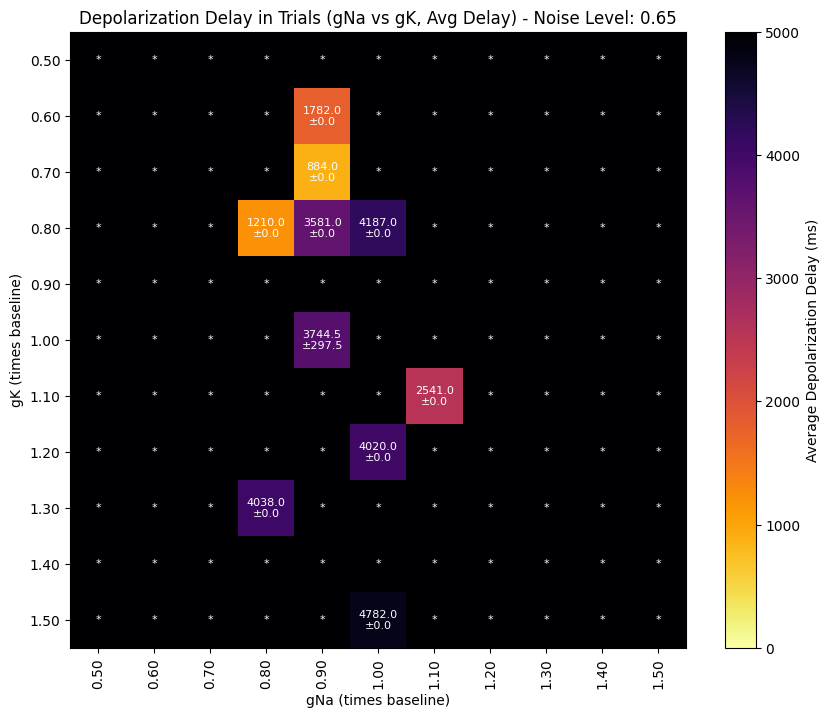
\includegraphics[width=\linewidth]{DPB_delay_matrices/DPB_delay_noise_0.65.png}
        \caption{} % Optional caption
    \end{subfigure}\hfill
    \begin{subfigure}{0.48\textwidth}
        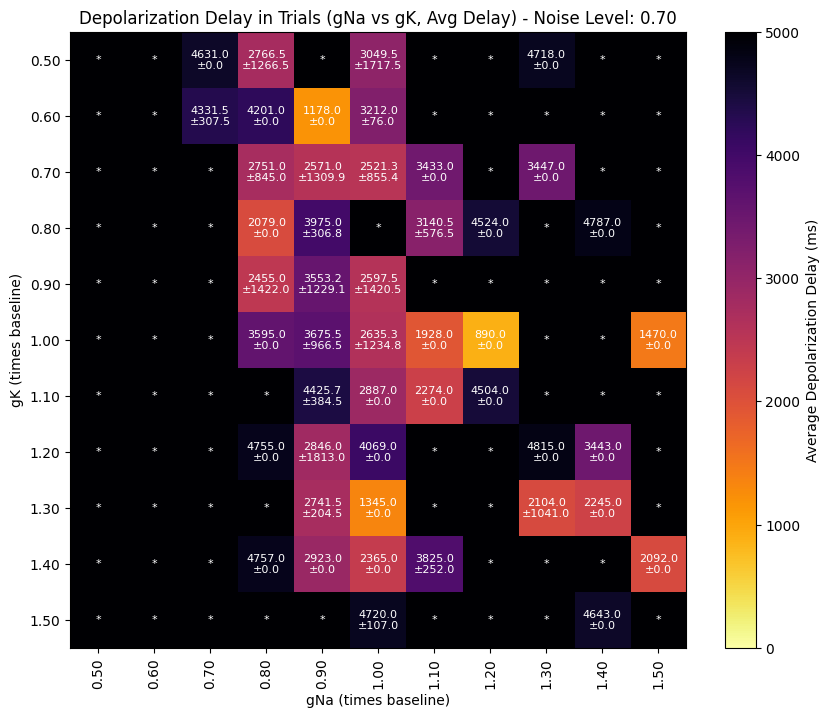
\includegraphics[width=\linewidth]{DPB_delay_matrices/DPB_delay_noise_0.70.png}
        \caption{} % Optional caption
    \end{subfigure}

    \bigskip % Adds vertical space between the rows

    % Row 2
    \begin{subfigure}{0.48\textwidth}
        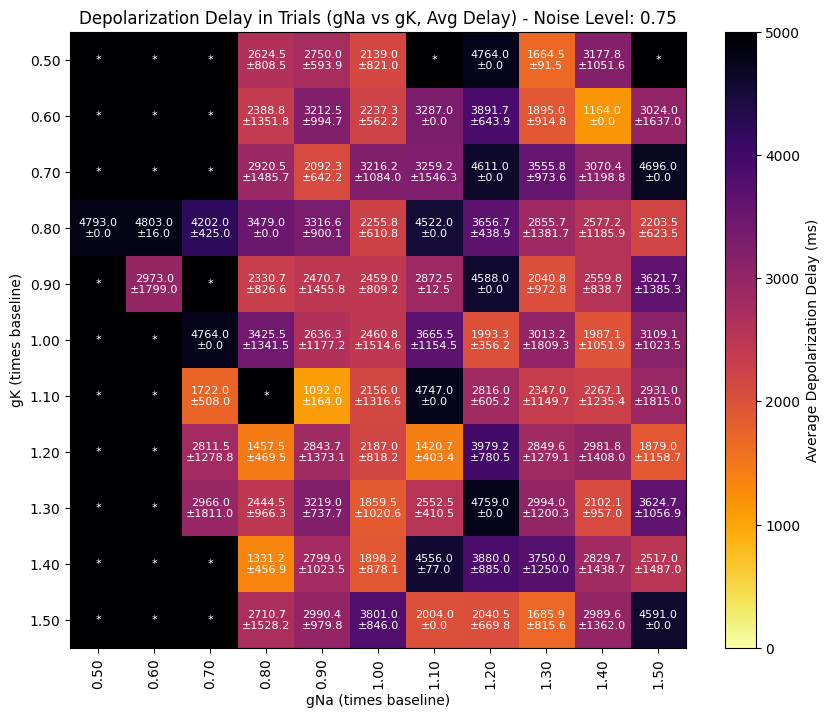
\includegraphics[width=\linewidth]{DPB_delay_matrices/DPB_delay_noise_0.75.png}
        \caption{} % Optional caption
    \end{subfigure}\hfill
    \begin{subfigure}{0.48\textwidth}
        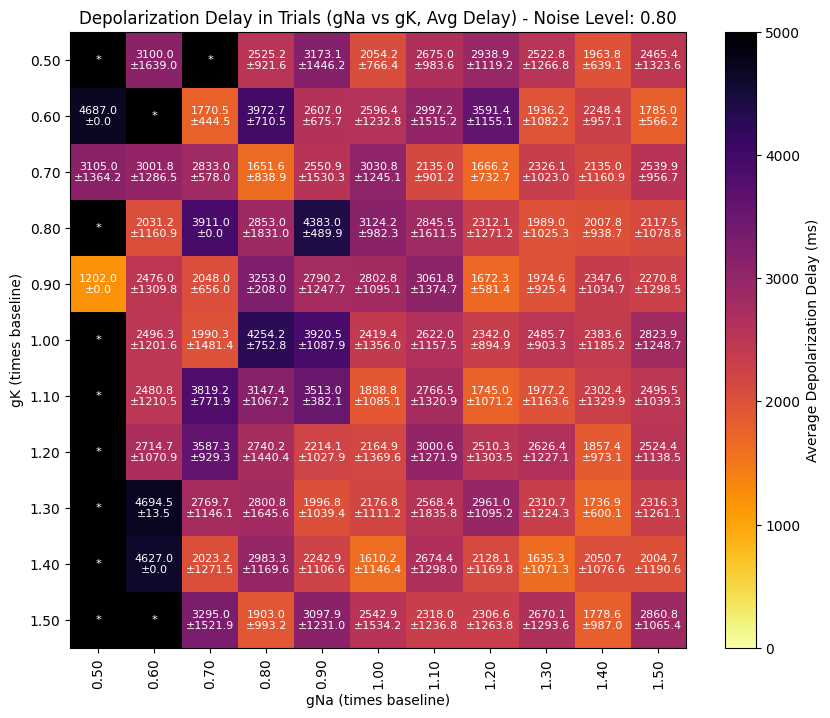
\includegraphics[width=\linewidth]{DPB_delay_matrices/DPB_delay_noise_0.80.png}
        \caption{} % Optional caption
    \end{subfigure}

    \caption[DPB delay matrices (all)]{Average delay + Standard deviation of DPB in trials where depolarization block events occurred for all tested noise conditions.
        The x-axis shows all the sodium conductance changes in pyramidal cells, whereas the y-axis shows the potassium conductance changes in pyramidal cells.
        Modifications to pyramidal cells were applied to all compartments.
        The color intensity shows the average delay, where high-intensity red equals a shorter delay in DPB events in a condition.
        An asterisk (*) is an indication that no DPB events occurred in the condition and is colorless.
        The images are labeled from low noise to higher noise (a through k), respectively.}\label{fig:dpb_delay_matrices_all}
\end{figure}

% Page 2
\begin{figure}[H] \ContinuedFloat% continue the figure from the previous page
    \centering
    % Row 3
    \begin{subfigure}{0.48\textwidth}
        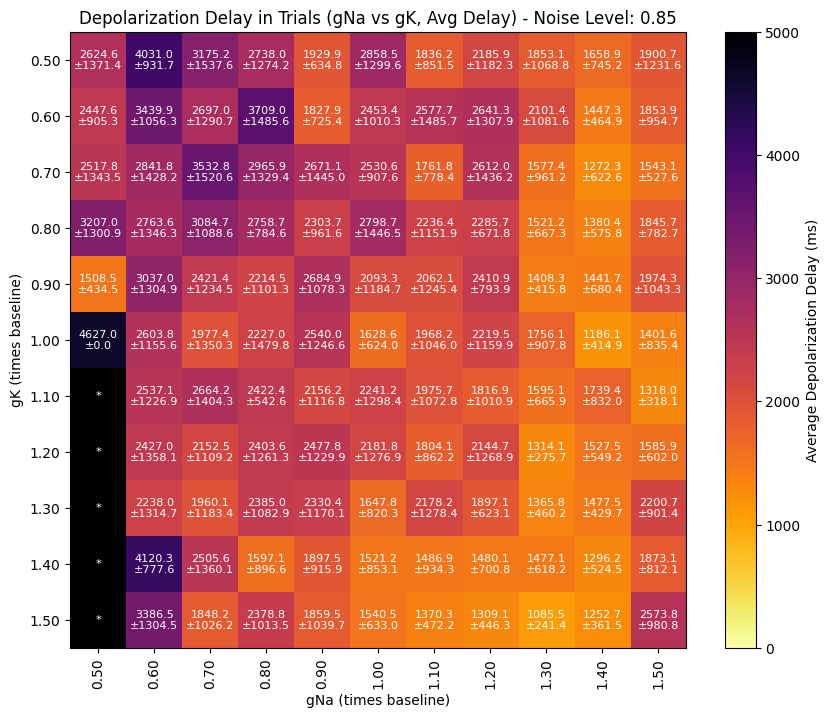
\includegraphics[width=\linewidth]{DPB_delay_matrices/DPB_delay_noise_0.85.png}
        \caption{} % Optional caption
    \end{subfigure}\hfill
    \begin{subfigure}{0.48\textwidth}
        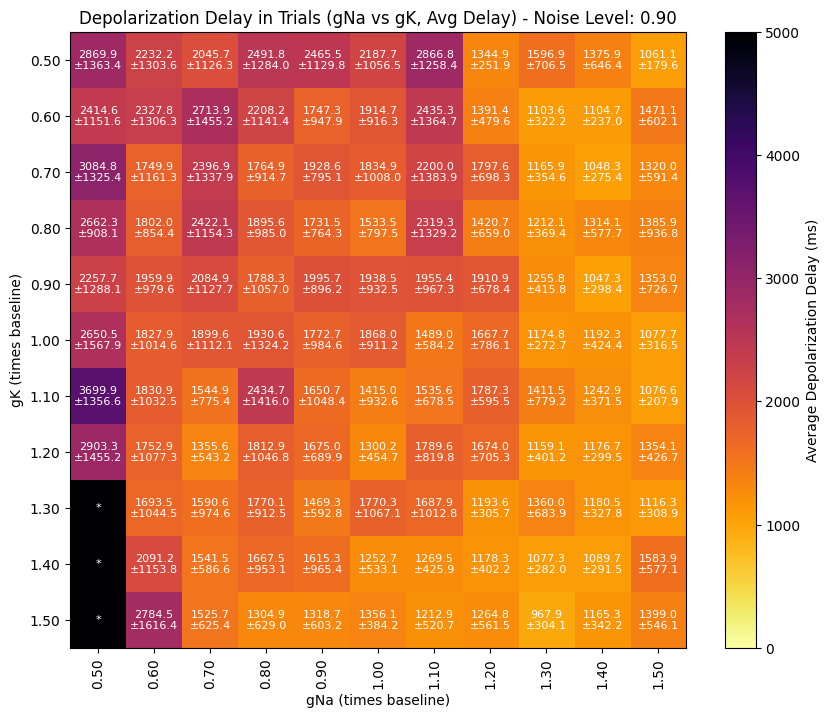
\includegraphics[width=\linewidth]{DPB_delay_matrices/DPB_delay_noise_0.90.png}
        \caption{} % Optional caption
    \end{subfigure}

    \bigskip % Adds vertical space between the rows

    % Row 4
    \begin{subfigure}{0.48\textwidth}
        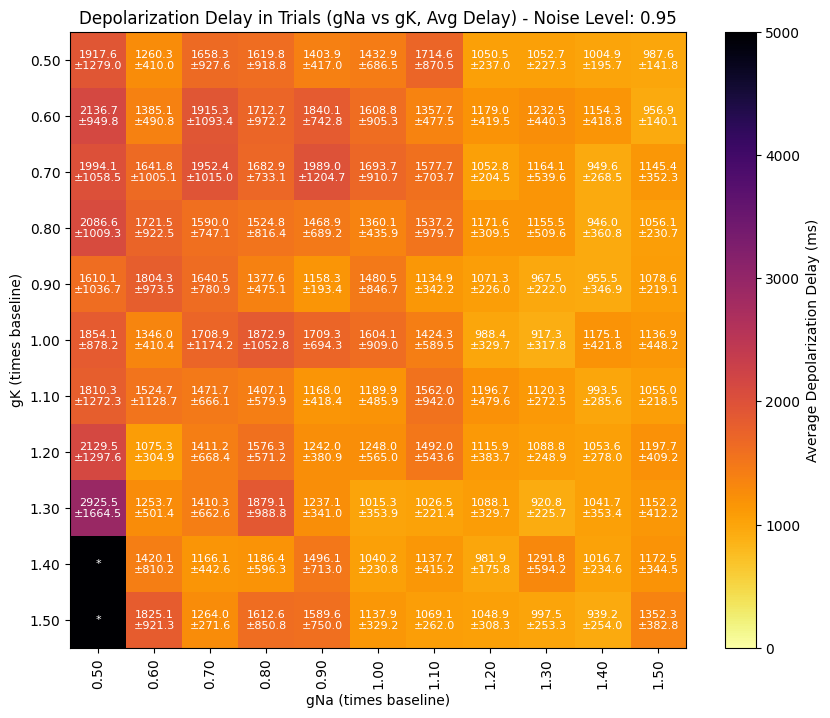
\includegraphics[width=\linewidth]{DPB_delay_matrices/DPB_delay_noise_0.95.png}
        \caption{} % Optional caption
    \end{subfigure}\hfill
    \begin{subfigure}{0.48\textwidth}
        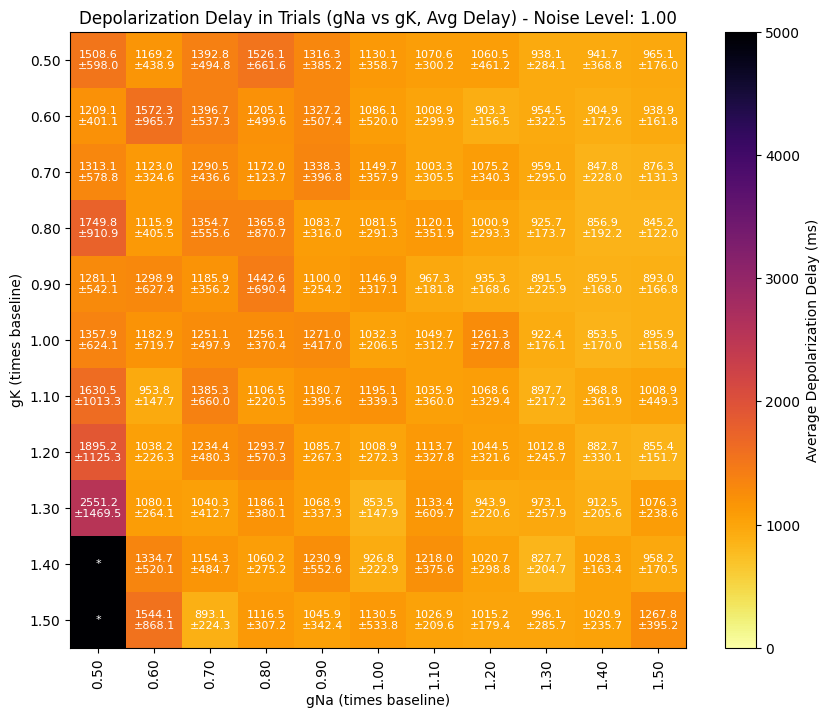
\includegraphics[width=\linewidth]{DPB_delay_matrices/DPB_delay_noise_1.00.png}
        \caption{} % Optional caption
    \end{subfigure}
\end{figure}

% Page 3
\begin{figure}[H] \ContinuedFloat% continue the figure from the previous page
    \centering
    % Row 5
    \begin{subfigure}{0.48\textwidth}
        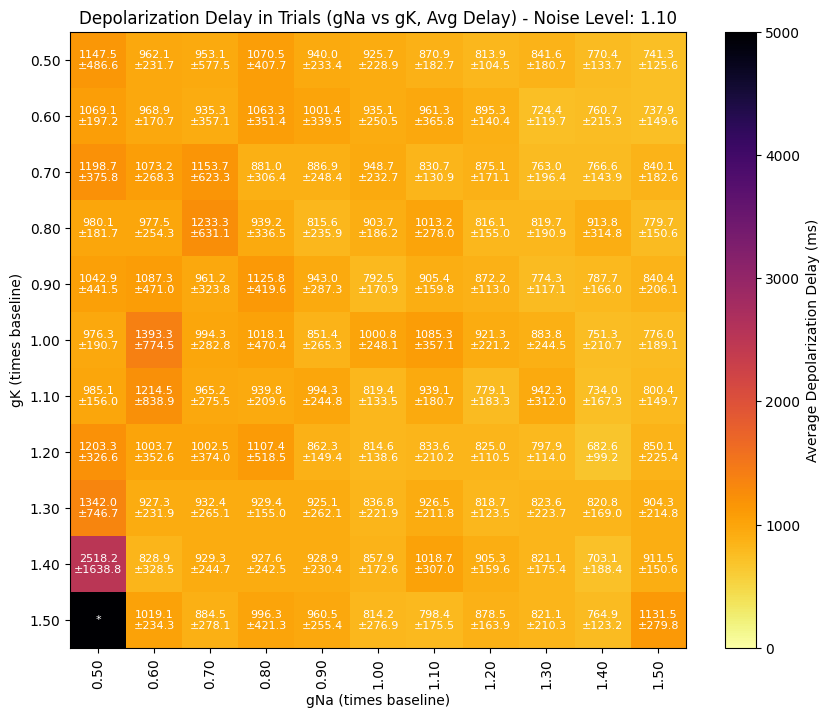
\includegraphics[width=\linewidth]{DPB_delay_matrices/DPB_delay_noise_1.10.png}
        \caption{} % Optional caption
    \end{subfigure}\hfill
    \begin{subfigure}{0.48\textwidth}
        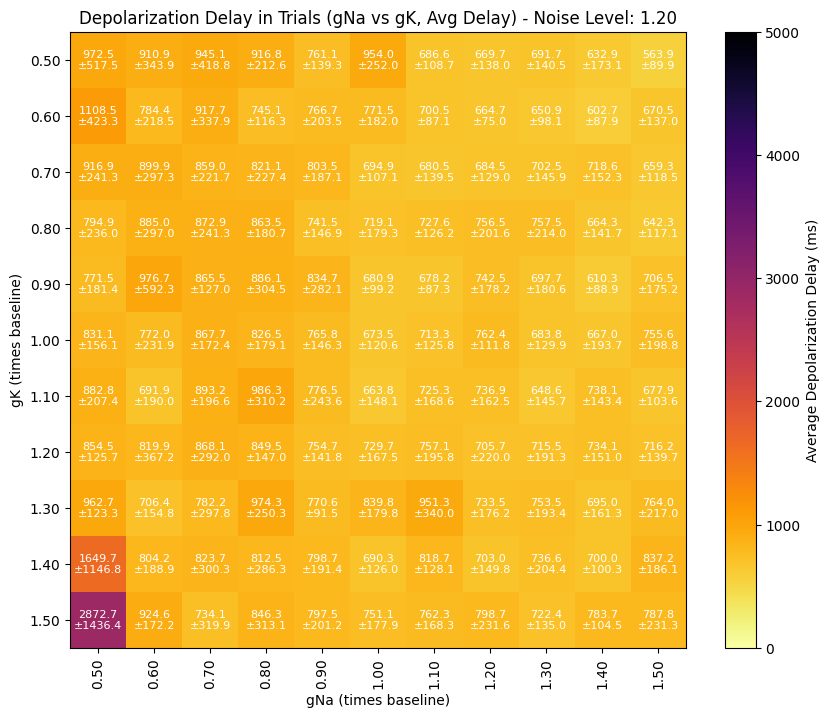
\includegraphics[width=\linewidth]{DPB_delay_matrices/DPB_delay_noise_1.20.png}
        \caption{} % Optional caption
    \end{subfigure}

    \bigskip % Adds vertical space between the rows

    % Row 6
    \begin{subfigure}{0.48\textwidth}
        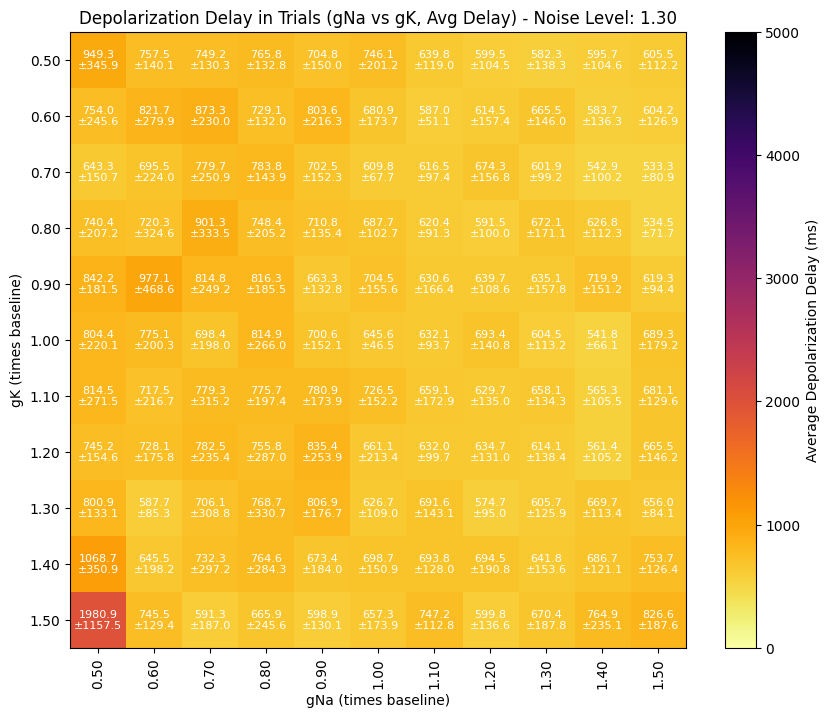
\includegraphics[width=\linewidth]{DPB_delay_matrices/DPB_delay_noise_1.30.png}
        \caption{} % Optional caption
    \end{subfigure}
    % Since the last row has only one image, you might adjust its position or add another sub-figure if needed.
\end{figure}
\pagebreak

\subsection{Recurrent connection matrices}\label{subsec:recurrent_connection_matrices}
% Page 1
\begin{figure}[H]
    \centering
    % Row 1
    \begin{subfigure}{0.48\textwidth}
        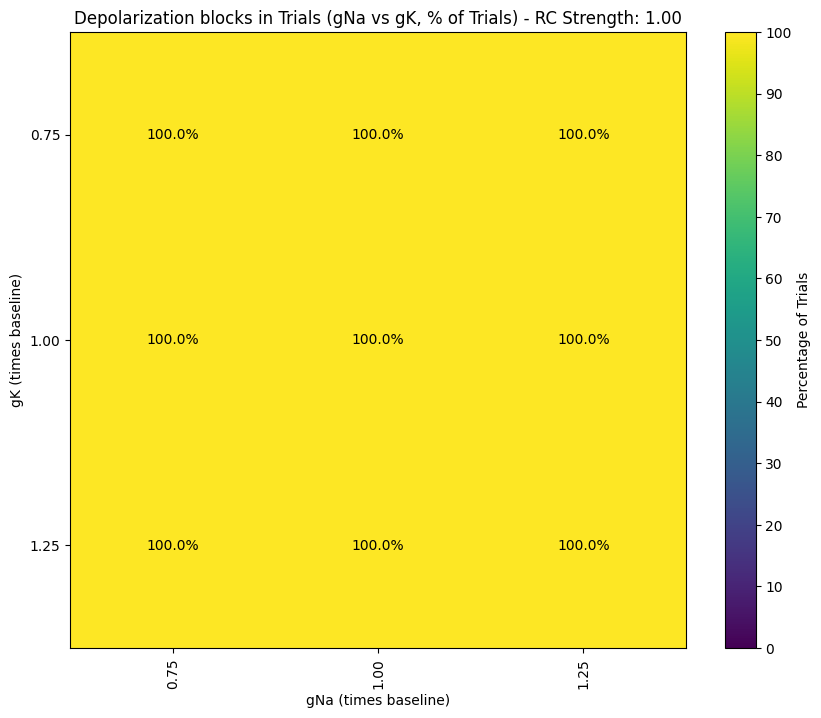
\includegraphics[width=\linewidth]{DPB_RC_Percentages/DPB_percentages_RC_1.00.png}
        \caption{} % Optional caption
    \end{subfigure}\hfill
    \begin{subfigure}{0.48\textwidth}
        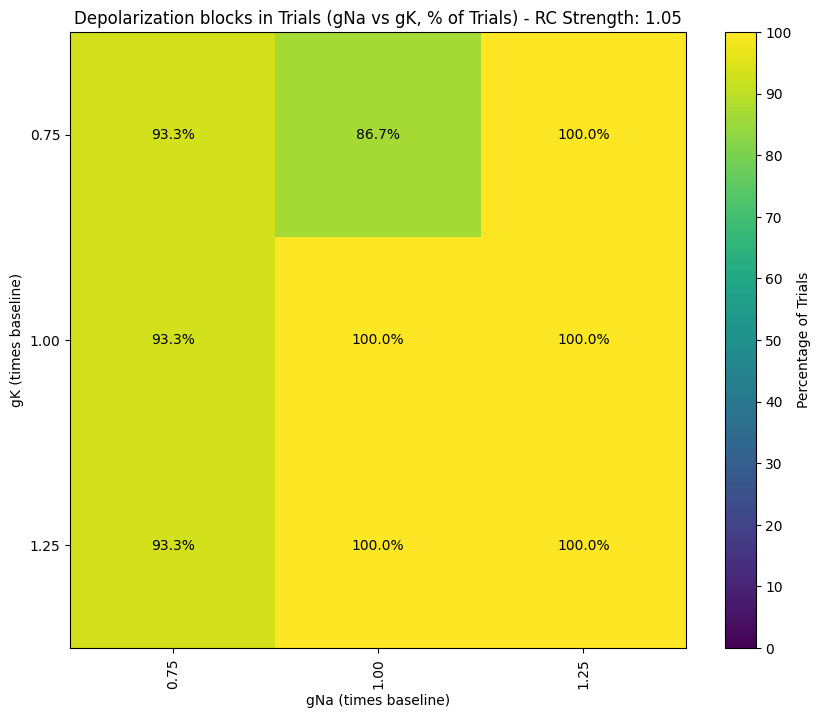
\includegraphics[width=\linewidth]{DPB_RC_Percentages/DPB_percentages_RC_1.05.png}
        \caption{} % Optional caption
    \end{subfigure}

    \bigskip % Adds vertical space between the rows

    % Row 2
    \begin{subfigure}{0.48\textwidth}
        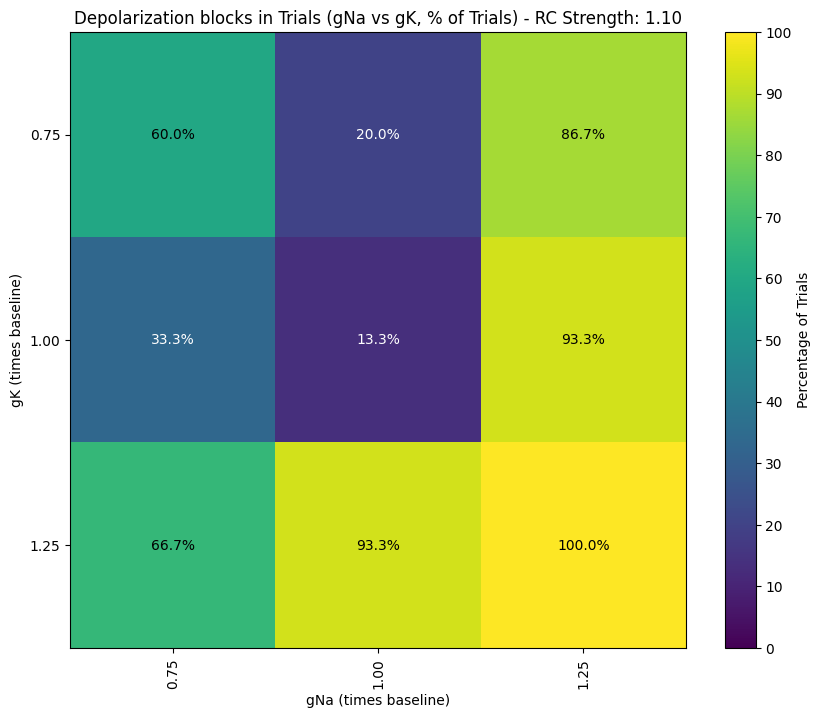
\includegraphics[width=\linewidth]{DPB_RC_Percentages/DPB_percentages_RC_1.10.png}
        \caption{} % Optional caption
    \end{subfigure}\hfill
    \begin{subfigure}{0.48\textwidth}
        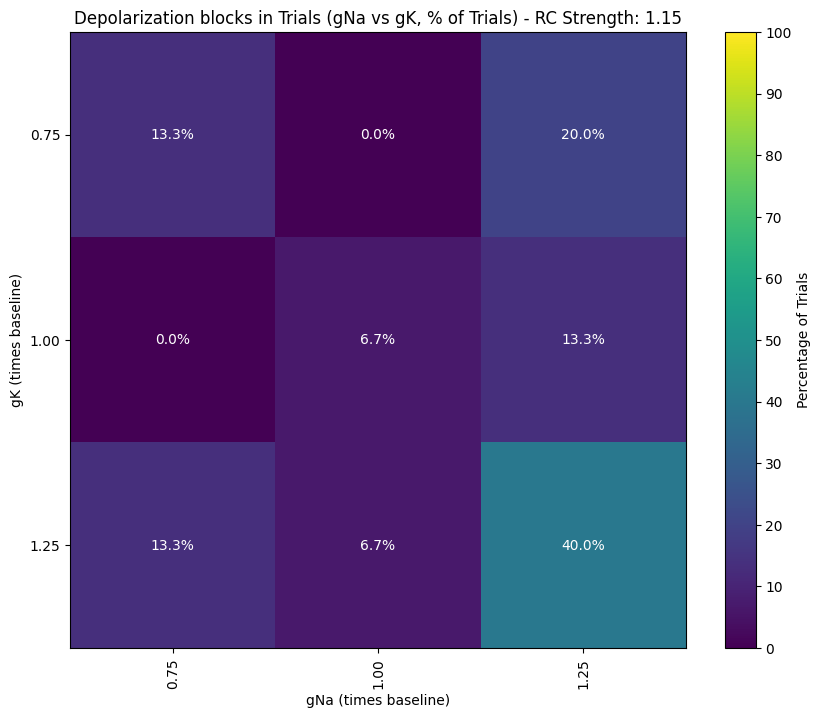
\includegraphics[width=\linewidth]{DPB_RC_Percentages/DPB_percentages_RC_1.15.png}
        \caption{} % Optional caption
    \end{subfigure}

    \caption[RC DPB percentage matrices (all)]{Percentage of trials where depolarization block events occurred for all tested noise conditions.
        The x-axis shows all the sodium conductance changes in pyramidal cells, whereas the y-axis shows the potassium conductance changes in pyramidal cells.
        Modifications to pyramidal cells were applied to all compartments.
        The color intensity shows the average delay, where high-intensity yellow equals higher percentage of DPB events in a condition.
        The images are labeled from low noise to higher noise (a through e), respectively.}\label{fig:rc_dpb_percentage_matrices_all}
\end{figure}

% Page 2
\begin{figure}[H] \ContinuedFloat% continue the figure from the previous page
    \centering
    % Row 3
    \begin{subfigure}{0.48\textwidth}
        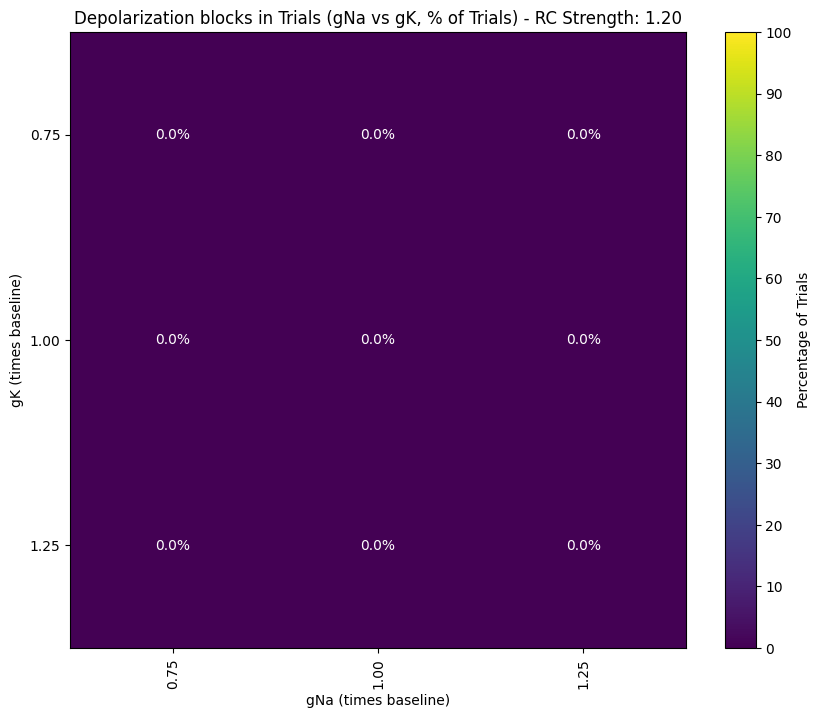
\includegraphics[width=\linewidth]{DPB_RC_Percentages/DPB_percentages_RC_1.20.png}
        \caption{} % Optional caption
    \end{subfigure}\hfill
\end{figure}